%%% fs-seim-optimistic - Optimistic approach

\label {fs-optimistic}

The main idea of our method is to represent stateful transformations as a sequence of a map and windowed grouping operations and handle out-of-order items within them. 

Following our approach, we make some assumptions about stream processing system, that is suitable for applying it. Such system must support meta-information on data items, allow cycles in the logical graph, and its set of predefined operations must be sufficient to express map and windowed grouping operations. Additionally, OOP indicators should be supported.

The ordering model of data items is defined at the beginning of this section. Then, we show that any stateful transformation can be implemented using the combination of windowed grouping and map operations. After that, we demonstrate an optimistic approach to handle out-of-order items within these operations. At the end of the section, the limitations of such technique are discussed.

\subsection{Ordering model}
We assume that there is a total order on data items. Ordering is preserved when an item is going through the operations. More precisely, the order of output items is the same as the order of corresponding input items. If more than one item is generated, they are inserted in output stream sequentially. Moreover, the output follows corresponding input but precedes the next item. The ordering model is shown in Figure ~\ref{ordering}. $F(x)$ is an arbitrary transformation. Replication and union are used to inject original unmodified items into the resulting stream to show the order between items. 

%% TODO: split and merge

\begin{figure}[htbp]
  \centering
  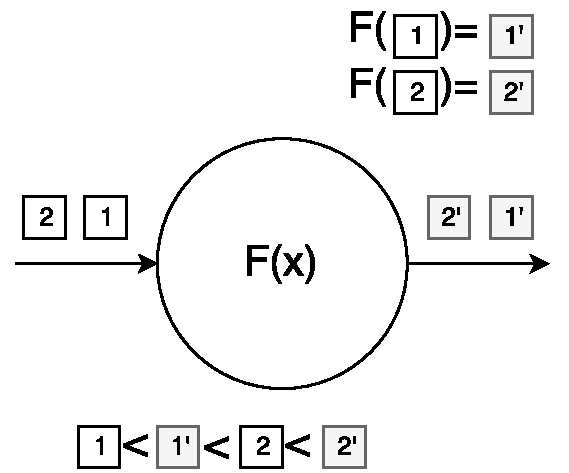
\includegraphics[width=0.5\textwidth]{pics/ordering}
  \caption{Ordering model}
  \label {ordering}
\end{figure}

\subsection{Semantics of map and windowed grouping operations}

\subsubsection{Map}
Map transforms input item into a sequence of its derivatives, according to a user-provided function $f$. This sequence can consist of any number of items or even be empty.

\subsubsection{Windowed grouping}
Windowed grouping is a stateful operation with a numeric parameter {\it window}. It is supposed that payloads of input items of grouping operation have key-value form. The state of this operation is represented by a set of buckets, one for each key. 

Windowed grouping has the following semantics:

\begin{itemize}
    \item Each input item is appended to the corresponding bucket
    \item The output of grouping operation is a window-sized tuple of the last items in the corresponding bucket. If bucket size is less than window, the output contains full bucket
\end{itemize}

The pseudocode is presented in Algorithm~\ref{group-semantics}. {\it Emit} function is called to send new items downstream.

\begin{algorithm}
\caption{Grouping semantics}
\label{group-semantics}
  \begin{algorithmic}[1]
    \Function{Insert}{$item$, $bucket$}
      \State \Call{Append}{$bucket, item$}
      \State $left \gets max(0, bucket_{length} - window)$
      \State $right \gets bucket_{length}$
      \State \Call{Emit}{$DataItem(bucket[left, right])$}
    \EndFunction
  \end{algorithmic}
\end{algorithm}

The following example illustrates the semantics of the windowed grouping operation. In this example, payloads of input items are represented as natural numbers: 1, 2, 3, etc. The hash function returns 1 if the number is even and 0 otherwise. If the window is set to 3, the output is:

\[(1), (2), (1|3), (2|4), (1|3|5), (2|4|6), (3|5|7), (4|6|8)...\]

\subsection{Stateful transformations using defined operations}
Figure~\ref{stateful-schema} shows the part of the logical pipeline, that can be used for stateful transformation. The input of windowed grouping operation is supposed to be ordered. There are several functional steps to produce output and update state. There are two cases of these steps:

\begin{itemize}
    \item When the first item arrives at grouping, it is inserted into the empty bucket. The grouping outputs single-element tuple, and then it is sent to the combined map. Combined map generates state object and sends it back to the grouping in the form of an ordinal key-value data item. The key of the state item is the same as in the item in tuple and value is the state. Combined map can generate some additional output and send it further down the stream.
    \item When the state item arrives at grouping, it is inserted in the tail of the corresponding bucket after the item that triggers state updating. The ordering model guarantees that the state item would be processed before the next item. Grouping outputs tuple with this item and the state. However, combine map filters out such tuple, because its last element is the state. This fact implies that the state has been already combined with the first item in the tuple.
    \item When new regular input item arrives at windowed grouping, it is inserted into the corresponding bucket's tail, because of the order assumptions. Additionally, the right ordering guarantees that input item is grouped into the tuple with previously generated state item. The next map operation combines new item and previous state into the new state item. After that, the new state item is returned to the grouping through the cycle. As in the first case, combined map can generate some additional output.
\end{itemize}

%% TODO: reordered tuple
%% TODO: both arrows in the same input

\begin{figure}[htbp]
  \centering
  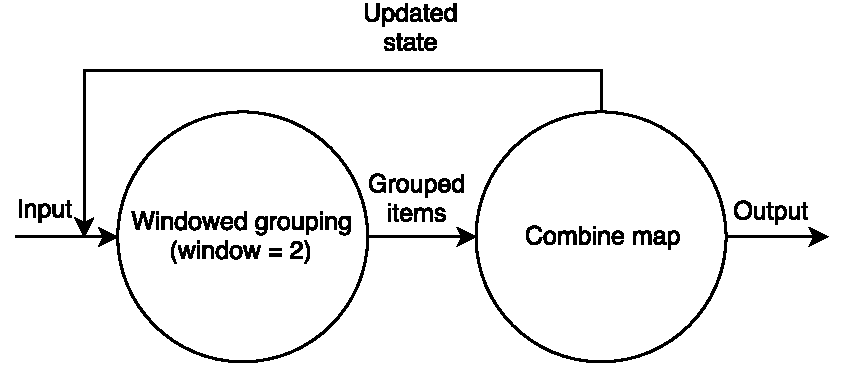
\includegraphics[width=0.48\textwidth]{pics/stateful-schema}
  \caption{The part of the logical pipeline for stateful transformation}
  \label {stateful-schema}
\end{figure}

The example of square matrix multiplication within proposed approach is shown in Figure ~\ref{matrix-example}. In this example, input items are represented as key-value pairs, where the key is the dimension of a matrix, and the value is the matrix itself. The reaction on three input matrices are the following:


%% 3 x 3 -> N x N
%% BAYESIAN INFERENCE
\begin{itemize}
    \item When the first matrix {\it A} arrives at grouping, it is put into the empty bucket for 3x3 matrices. After that, the single-element tuple with matrix {\it A} is sent to combine map operation. Combine map creates state object for matrix {\it A}, which is just {\it A} itself. In the last step, state item is sent back to grouping, and it is inserted right after item for matrix {\it A}
    \item Matrix {\it B} is arrived and inserted into the bucket right after state item. The tuple containing state item and item for matrix {\it B} is sent to combine map. Combine map multiplies matrix in the state by matrix {\it B}. The result of this operation is matrix {\it AB}. New state item for matrix {\it AB} is created and sent back to the grouping. It is inserted in bucket right after item with matrix {\it B}
    \item Matrix {\it C} is arrived and went through the pipeline in a similar way as matrix {\it B}
\end{itemize}

\begin{figure}[htbp]
  \centering
  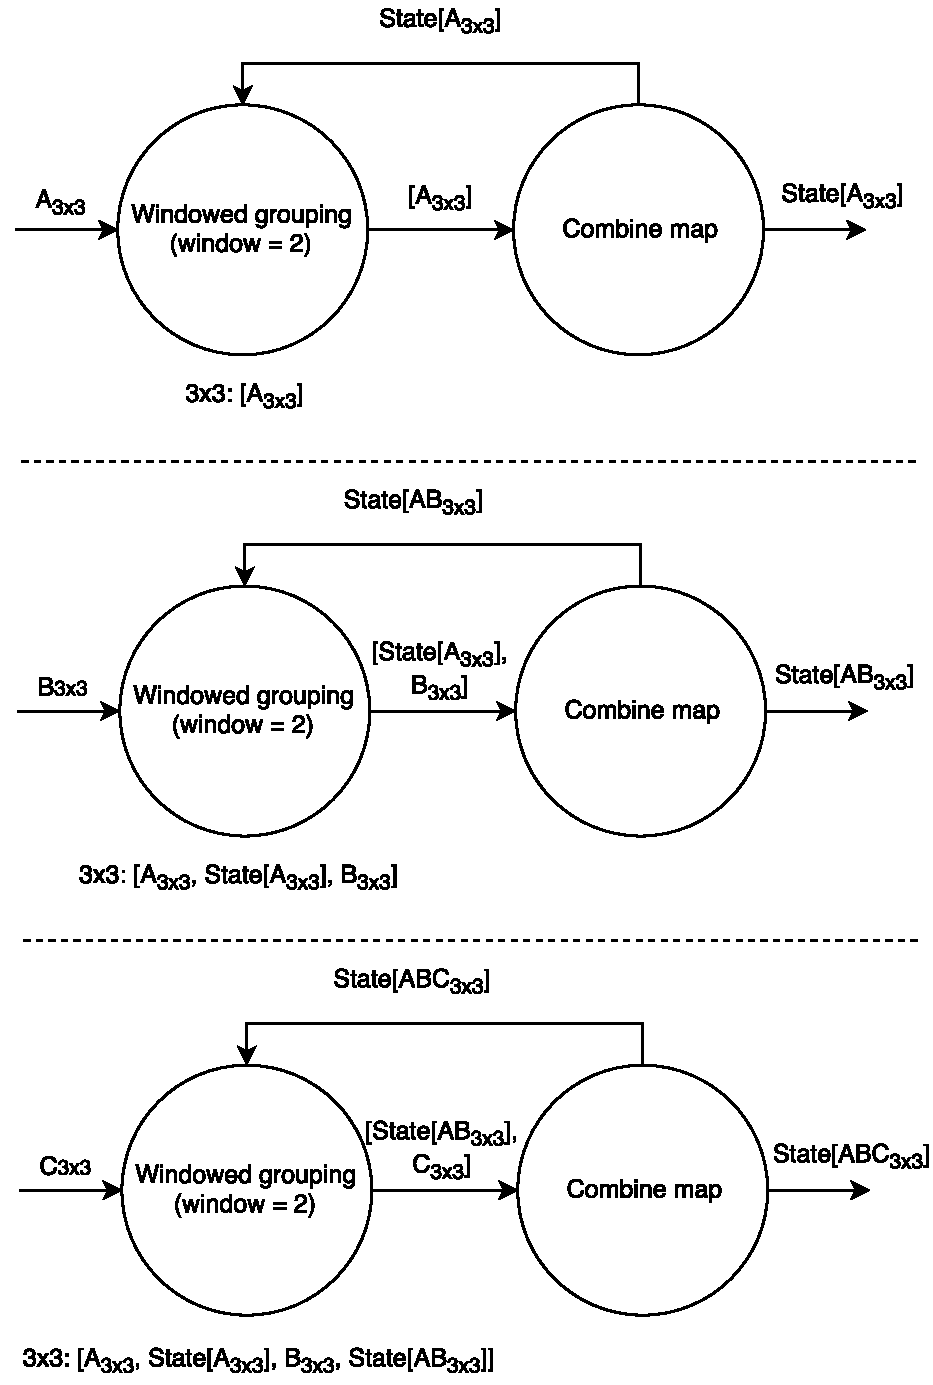
\includegraphics[width=0.48\textwidth]{pics/matrix-example}
  \caption{Matrix multiplication example}
  \label {matrix-example}
\end{figure}

\subsection{Handling out-of-order events}
When we introduce the model for stateful operations, we assume that all items arrive at grouping in the right order. However, as it was shown above, it is not possible in practice without additional buffering. We propose the following approach to handle events in grouping:

\begin{itemize}
    \item If an item arrives in order, it is processed as usual
    \item If two items are out-of-order, and the grouping observes the second one then it is inserted into the corresponding bucket at the position defined by the meta-information. After that, tuples, which contain new item are generated and sent further down the stream. At the same time, for tuples, that has been produced but became invalid, {\it tombstones} are sent
\end{itemize}

Tombstones are ordinal data items but with a special flag in meta-information. This flag means that tuples with such meta-information are invalid, and they should not leave the system. Tombstones have the same payloads as invalid items in order to go through the same path in the computational pipeline.

The pseudocode of the grouping is shown in Algorithm \ref{group-insert}. The functions accept new element, depending on its type. They also receive a bucket for element's hash. {\it Emit} function is called to send new items downstream.

\begin{algorithm}
\caption{Implementation of grouping semantics}
\label{group-insert}
  \begin{algorithmic}[1]
    \Function{InsertTombstone}{$item$, $bucket$}
      \State $cleanPosition \gets lowerBound(item, bucket)$
      \ForAll{$group: group \cap cleanPosition \neq \emptyset$}
        \LineComment{Send tombstones for invalid groups}
        \State \Call{Emit}{$DataItem_{tomb}(group)$}
      \EndFor

      \State \Call{Remove}{$bucket, cleanPosition$}

      \ForAll{$group: group \cap cleanPosition \neq \emptyset$} 
        \LineComment{Emit new groups that appeared after collapse}
        \State \Call{Emit}{$DataItem(group)$} 
      \EndFor
    \EndFunction

    \State

    \Function{InsertRegular}{$item$, $bucket$}
      \State $insertPosition \gets lowerBound(item, bucket)$
      \ForAll{$group: group \cap insertPosition \neq \emptyset$} 
        \LineComment{Send tombstones for groups that would disappear}
        \LineComment{after insert}
        \State \Call{Emit}{$DataItem_{tomb}(group)$} 
      \EndFor
      
      \State \Call{Insert}{$bucket, insertPosition$}

      \ForAll{$group: group \cap insertPosition \neq \emptyset$} 
        \LineComment{Emit new groups}
        \State \Call{Emit}{$DataItem(group)$} 
      \EndFor
    \EndFunction
  \end{algorithmic}
\end{algorithm}

This technique guarantees that all correct tuples are eventually produced. However, invalid ones are also generated. Therefore, there is a need for {\it barrier} at the pipeline's sink, that filters invalid items when corresponding tombstones arrive. The barrier is partially flushed for some meta-information interval when there is a guarantee that there are no any out-of-order items and tombstones further up the stream for this range. This guarantee can be provided by punctuations or low watermarks, as it is implemented in the most stream processing systems. The fundamental idea behind this approach is to shift blocking as far as possible down the stream. Notably, this is the only buffer in the whole system, unlike existing solutions.

The pseudocode for the barrier is shown in Algorithm~\ref{barrier-insert}. The function {\it Insert} is called upon new item's arrival, {\it Punctuation} - on punctuation's. 

\begin{algorithm}
\caption{Barrier}
\label{barrier-insert}
  \begin{algorithmic}[1]
    %% TODO: pretty print
    \State $buffer \gets \emptyset$

    \State

    \Function{Insert}{$item$}
      \State $position \gets lowerBound(item, buffer)$
      \If {$isTombstone(item)$}
        \State \Call{Remove}{$buffer, position$}
      \Else
        \State \Call{Insert}{$buffer, position$}
      \EndIf
    \EndFunction

    \State

    \Function{Punctuation}{$time$}
      \ForAll{$item:  item \in buffer \And item_{ts} < time$}
        \State \Call{Emit}{$item$}
        \State \Call{Remove}{$item$, $buffer$}
      \EndFor
    \EndFunction
  \end{algorithmic}
\end{algorithm}

\subsection{Advantages and limitations}
The proposed architecture's performance depends on how often reorderings are observed during the runtime. In the case when the order naturally preserved there is almost no overhead: when the watermark arrives, all computations are already done. The probability of reordering could be managed on a business-logic level and optimized by the developer. In experiments section it is shown that the computational nodes count is one of such parameters.

Regarding the weaknesses, this method can generate additional items, which lead to extra network traffic and computations. Experiments, which are shown in the section~\ref{fs-experiments} demonstrate that the number of extra items is low.
